\subsection{Throughput}
This test was designed to measure the transmission performance of Bluetooth in the context of a long lasting connection to a single other device such as the exchange of a picture or video.
The metric of interest was throughput, which is defined as the number of bytes transferred per second.

A single round of test worked by connecting two devices, a client and a server and performing 20 transfers using the same connection.
Each of the 20 transfers measured the time needed to send a test payload of 2000 kbytes from the server to the client.
The pseudo code for client and server is shown in Algorithm \ref{pseudo:tr_client} and \ref{pseudo:tr_server}.
When 20 transfers were completed the data collected was saved for further processing.

\begin{algorithm}
	\begin{algorithmic}[1]
  		\caption{client pseudocode}
  		\label{pseudo:tr_client}
		\State $socket \leftarrow connectToServer()$
		\State $results \leftarrow emptyList()$
		\For{$i=1$ to $20$}
		    \State $T_0 \leftarrow nanotime()$ \Comment current time in nanoseconds
			\State $data \leftarrow socket.read(2048000)$ 
			\State $T_1 \leftarrow nanotime()$
			\State $list.add(T_1 - T_0)$
		\EndFor
		\State \Return $results$
  	\end{algorithmic}
\end{algorithm}

\begin{algorithm}
	\begin{algorithmic}[1]
  		\caption{server pseudocode}
  		\label{pseudo:tr_server}
  		\State $socket \leftarrow serverSocket.accept()$
		\Repeat
		    \State $data \leftarrow randomByteArray(2048000)$
            \State $socket.write(data)$
		\Until{client closes the connection}
		\State \Return $results$
  	\end{algorithmic}
\end{algorithm}

In order to collect a meaningful amount of data the test was performed multiple times using different devices as client and server.
The devices used along with the number of measurements performed are shown in Table \ref{table:tr-measurements}.

\begin{figure}[h]
  \centering
  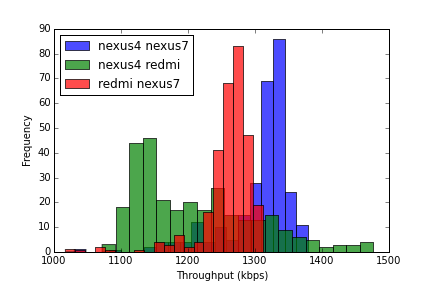
\includegraphics[width=1.0\textwidth]{application/img/tr-distribution.png}
  \caption{Distribution of throughput for each pair of devices tested.}
  \label{figure:tr-distribution}
\end{figure}

\begin{table}[ht]
\centering
\begin{tabular}{llll}
\hline
Client        & Server      & Number of rounds &  Failed  \\ \hline
Nexus 4       & Nexus 7     & 15               & 1        \\
Redmi         & Nexus 7     & 15               & 0        \\
Nexus 4       & Redmi       & 15               & 0        \\
\hline
\end{tabular}
\caption{Devices used to compute troughput and number of rounds}
\label{table:tr-measurements}
\end{table}

For each measurement $(T_0, T_1, N)$ collected, the throughput in $kbps$ was computed as 
\[\frac{N*8/1000}{T_1 - T_0}\]
where $N$ was the number of bytes, $T_0$ was the initial time and $T_1$ was the final time.

The distribution of throughput for each pair tested, is shown in Figure \ref{figure:tr-distribution}.

The average throughput, computed as the mean of all the values, was $1258 kpbs$ which is a value sufficient to send pictures taken from a modern smartphone in just a few seconds.

